\section{Racine RPL}\label{sec:work-rpl-root}
\renewcommand{\rightmark}{Racine RPL}

    Dans la topologie choisie à la section \ref{sec:archi-topologie}, une racine RPL est la plateforme de développement Zolertia RE-Mote Rev.B à laquelle la carte d'interface du RN2483 a été raccordée par des câbles de prototypage. La figure~\ref{fig:work-montage} illustre le raccordement entre le RN2483 et le Zolertia.
    
    \begin{figure}[H]
        \centering
        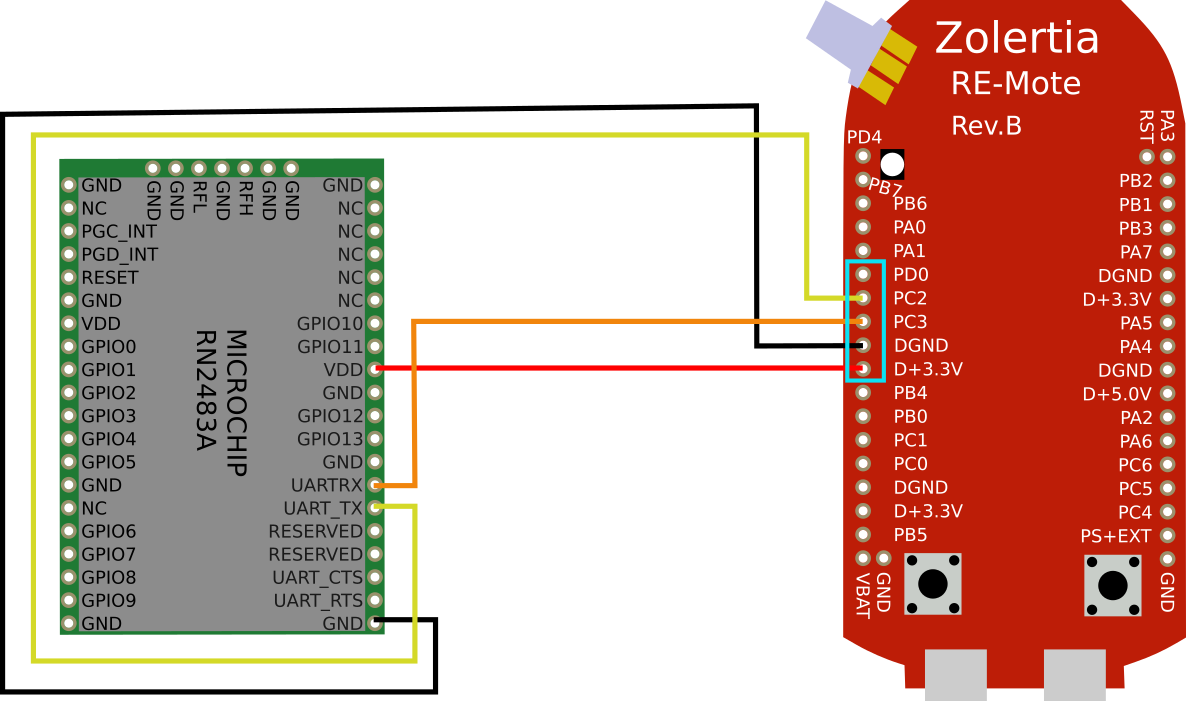
\includegraphics[scale=0.35]{res/pictures/montage.png}
        \caption{Schéma du raccordement du RN2483 au Re-Mote}
        \label{fig:work-montage}
    \end{figure}

    Comme l'indique la table~\ref{table:work-pin-description} de description des pins, les pins PC2 et PC3 utilisés pour la connexion ne sont pas ceux défini pour l'usage d'une connexion UART. Ces pins sont choisis pour la connexion UART car ils sont accessibles à l'exterieur du boitier de la plateforme par un connecteur.
    
    Pour que la connexion UART avec le RN2483 soit possible via les pins choisis, des modifications 
    dans Contiki du fichier de configuration de la plateforme sont nécéssaires.
    Ainsi, les valeurs des macros suivantes ont été modifiées dans le fichier \texttt{arch/cpu/cc2538/cc2538-conf.h}:
    \begin{itemize}
        \item \texttt{UART1\_CONF\_BAUD\_RATE} est définie à $57600$ qui est le baudrate par défaut du RN2483
        \item \texttt{UART1\_RX\_PIN} est définie à $2$
        \item \texttt{UART1\_TX\_PIN} est définie à $3$
    \end{itemize}

    Comme pour l'implémentation de la racine LoRa, celle de la racine RPL est réalisée en 3 couches.

\subsection*{Couche physique}
    %todo
\subsection*{Couche MAC}
    %todo
\subsection*{Couche IP}
    %todo
% Please add the following required packages to your document preamble:
% \usepackage{graphicx}
% \usepackage[table,xcdraw]{xcolor}
% If you use beamer only pass "xcolor=table" option, i.e. \documentclass[xcolor=table]{beamer}
\begin{table}[]
    \centering
    \makebox[\textwidth]{%
    \begin{tabular}{|l|l|l|l|}
    \hline
    \rowcolor[HTML]{C0C0C0} 
    Pin & Default name       & MC  & Description                                                                            \\ \hline
    4   & UART0.RX           & PA0 & Connected to the CP2104 USB-to-serial converter                                        \\ \hline
    5   & UART0.TX           & PA1 & Connected to the CP2104 USB-to-serial converter                                        \\ \hline
    6   & GPD0/I2C.Interrupt & PD0 & Generic pin, may be used as auxiliary pin for I2C/SPI                                  \\ \hline
    7   & I2C.SDA            & PC2 & \multicolumn{1}{p{10cm}|}{GPIO 20 mA output capability, pull-up. Shared with the RTCC and on-board low-power PIC} \\ \hline
    8   & I2C.SCL            & PC3 &  \multicolumn{1}{p{10cm}|}{GPIO 20 mA output capability, pull-up. Shared with the RTCC and on-board low-power PIC} \\ \hline
    9   & DGND               & N/A & Digital Ground                                                                         \\ \hline
    10  & D+3.3              & N/A & 3.3VDC output pin                                                                      \\ \hline
    11  & CC1200.GPIO0       & PB4 &  \multicolumn{1}{p{10cm}|}{CC1200 GPIO0 pin. If RF switch disables sub-GHz is available for other purposes}        \\ \hline
    12  & CC1200.GPIO2       & PB0 &  \multicolumn{1}{p{10cm}|}{CC1200 GPIO2 pin. If RF switch disables sub-GHz is available for other purposes}        \\ \hline
    13  & UART1.RX           & PC1 &  \multicolumn{1}{p{10cm}|}{GPIO 20 mA output capability, no pull-up or pull-down.}                                 \\ \hline
    14  & UART1.TX           & PC0 &  \multicolumn{1}{p{10cm}|}{GPIO 20 mA output capability, no pull-up or pull-down.  }                               \\ \hline
    \end{tabular}%
    }
    \caption{Extrait de la table de descrition des pins.~\cite{zolertia-remote:datasheet}}
    \label{table:work-pin-description}
    \end{table}